\section{Ray Tracing}

The idea behind ray tracing the reverse process of what we did until now. We start by shooting rays through each pixel in our image.
\begin{center}
	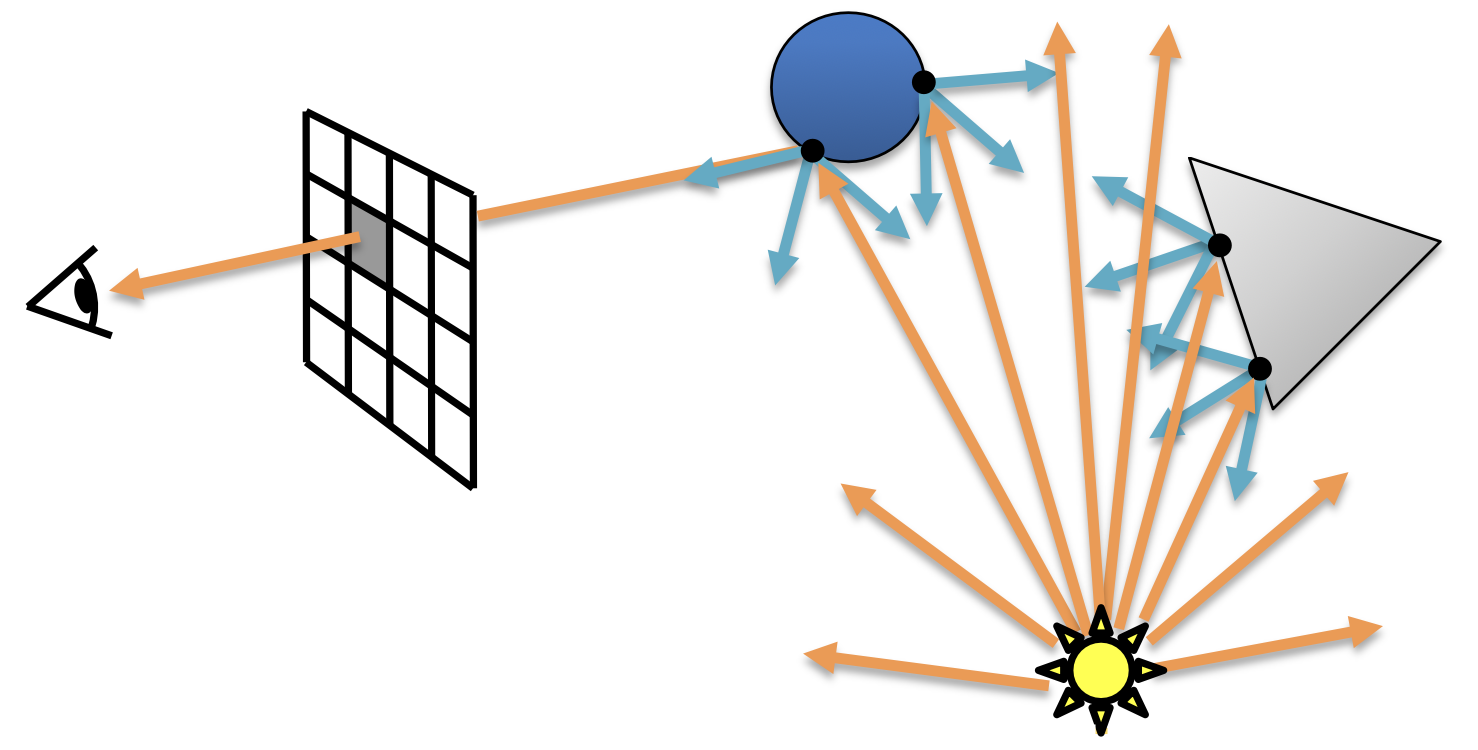
\includegraphics[width=\linewidth]{ray_tracing.png}
\end{center}

The first versions of ray tracing stoped at the first intersection with an object and then evaluated the illumination model for this point (also called \textbf{ray casting}). Nowadays \textbf{recursive ray tracing} calculates refractions of that initial ray until we arrive at the light source.


\subsection{Forward Ray Tracing}

Forward ray tracing would theoretically start at the light source and trace each ray until it hits the camera. This is not very efficient as most rays will never hit the camera.


\subsection{Backward Ray Tracing}

Backward ray tracing therefore does it the other way round. It traces rays from the camera into the scene until arriving at a light source. This easily solves some of the problems we previously encountered, e.g. hidden surface problem or transparency. When arriving at a object we calculate the lighting model for this point by casting additional rays depending on the type of surface (diffuse, glossy, specular). Additionally to determine shadows, we cast a ray towards the light source, if the ray arrives at the light source our point does not lie inside a shadow.
\begin{center}
	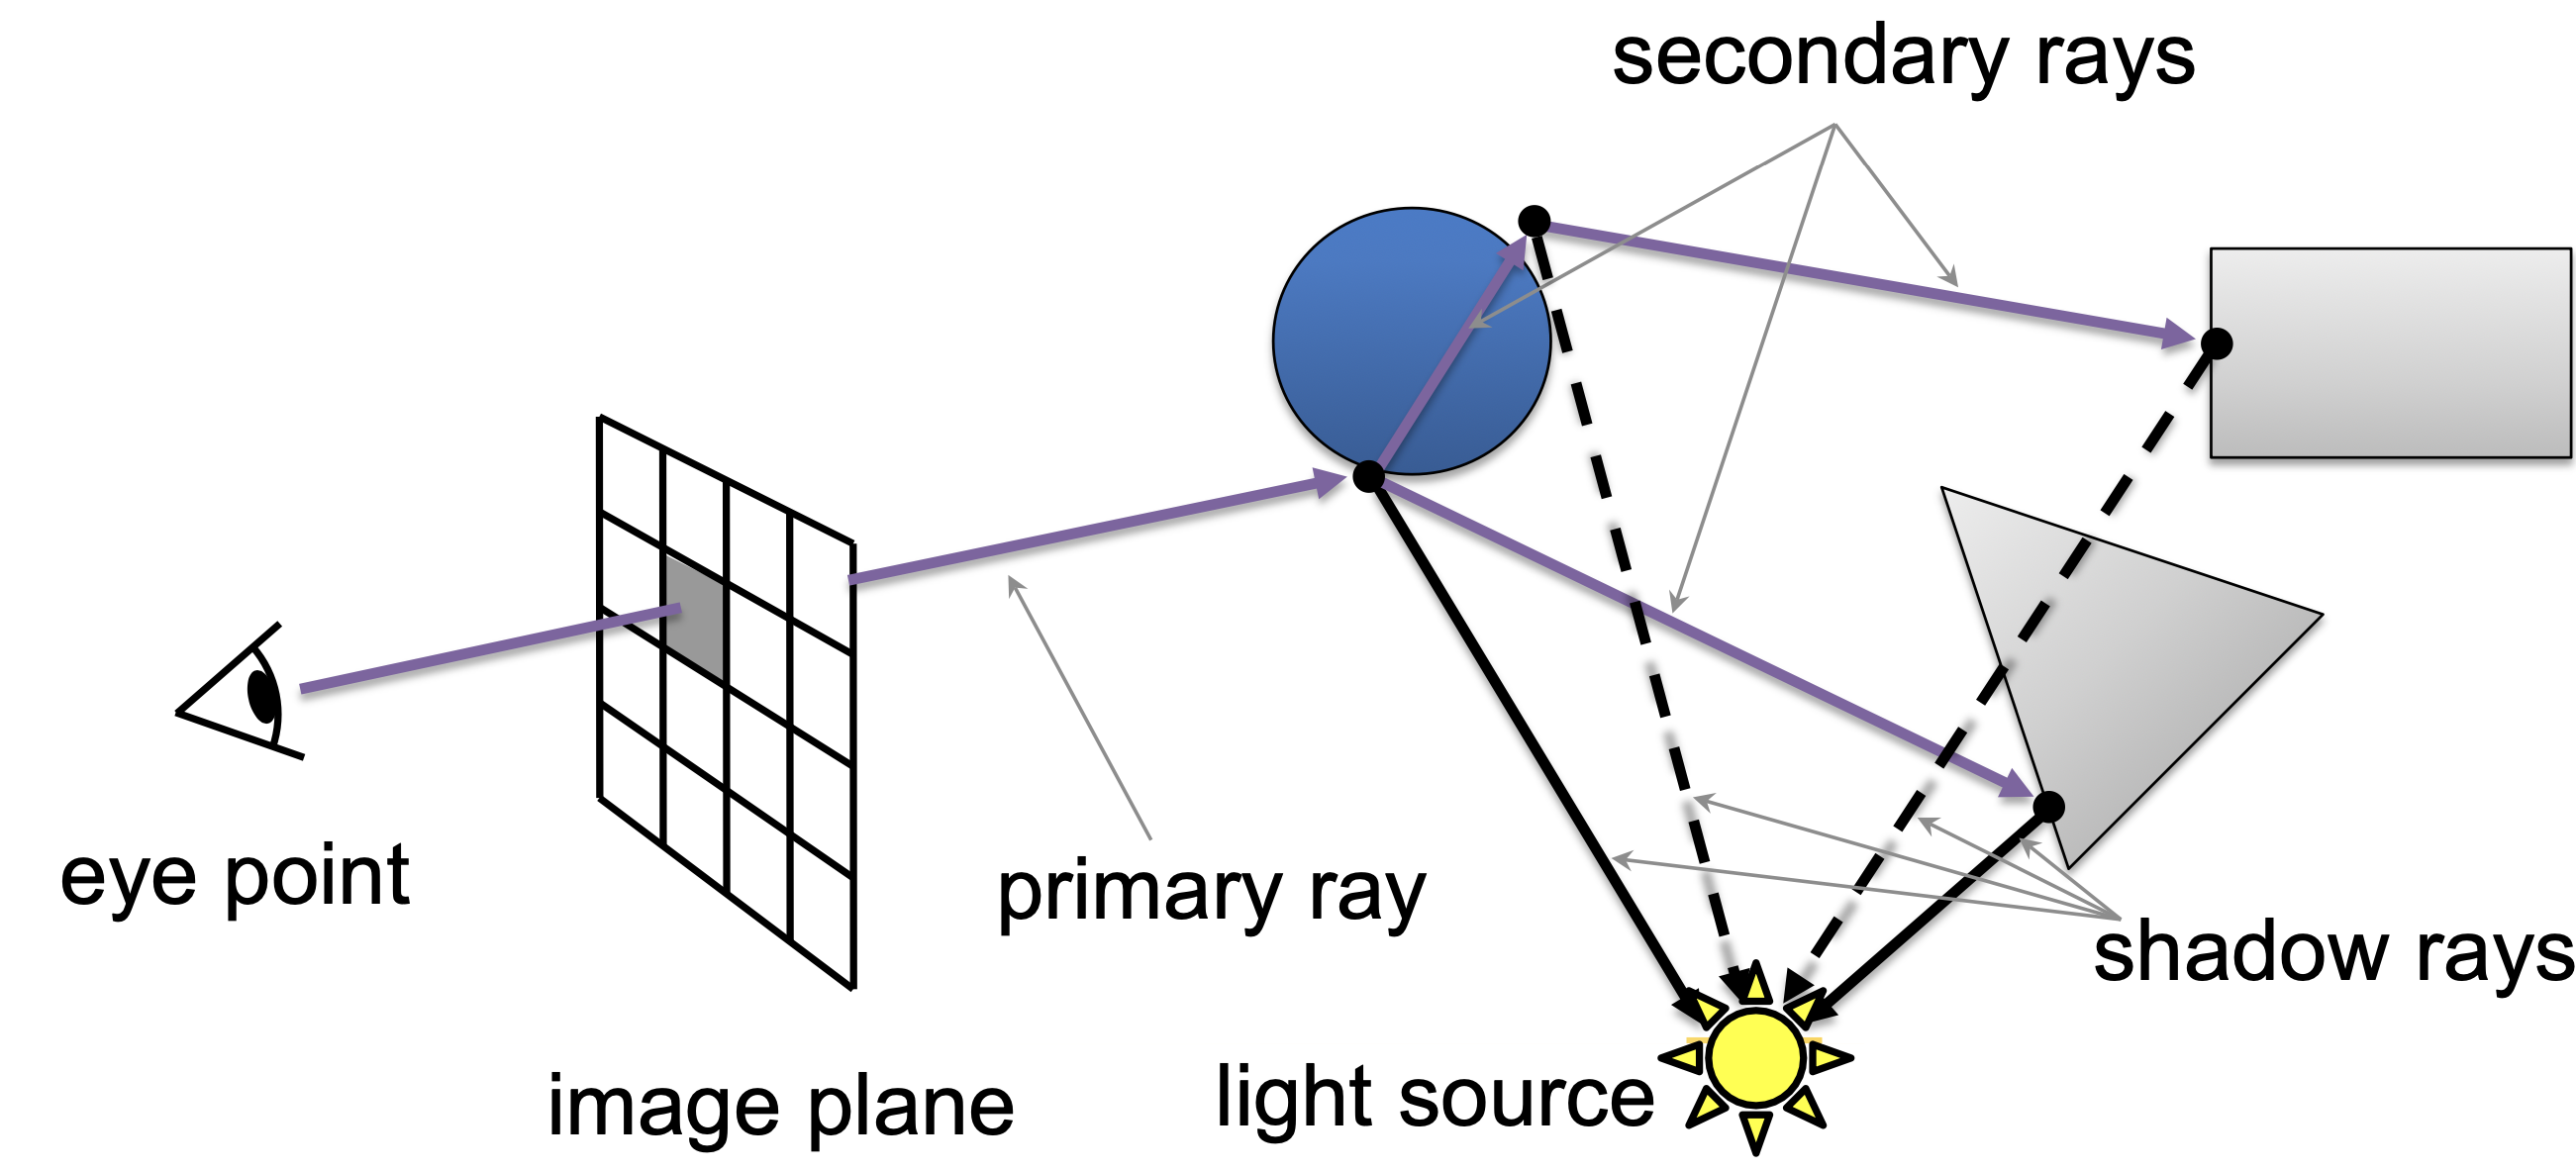
\includegraphics[width=\linewidth]{backward_raytracing.png}
\end{center}

The basic pipeline therefor consists of the following steps:
\begin{itemize}
	\item Ray Generation
	\item Intersection
	\item Shading
\end{itemize}

This three stages get repeated over and over. If we shoot multiple ray per pixel (supersampling) we not only improve the quality, but also implement anti-aliasing. \medskip

The ray equation is given by:
$$r(t) = o + td$$

$o$ is the origin of the ray and $d$ the direction. Using this we can calculate the intersection with various types of primitives, e.g. triangles or spheres.

\subsection{Shading}

We already said that physically correct shading is too expensive. Therefore we need to simplify by making some assumptions. We assume that there are different types of surface reflectance: diffuse, specular, ambient and transparency terms. Further we use the shadow ray to determine if a point is illuminated.
